\documentclass[12pt, twoside]{article}
\usepackage[francais]{babel}
\usepackage[T1]{fontenc}
\usepackage[latin1]{inputenc}
\usepackage[left=8mm, right=8mm, top=8mm, bottom=8mm]{geometry}
\usepackage{float}
\usepackage{graphicx}
\usepackage{array}
\usepackage{multirow}
\usepackage{amsmath,amssymb,mathrsfs}
\usepackage{textcomp}
\usepackage{soul}


\pagestyle{empty}
\begin{document}

\begin{flushright}
$2^{de}5$
\end{flushright}
\section*{\center{Devoir maison 2}}


\textit{Devoir � rendre sur feuille double grand format petits carreaux pour le
\ul{samedi 18 octobre 2008}. Toutes les r�ponses seront fournies sur votre
copie double, pour l'exercice 1, rendre le tableau.}

\bigskip
\textbf{Exercice 1:}
Remplir le tableau de la deuxi�me page.


\bigskip
\textbf{Exercice 2:}
\begin{center}
	  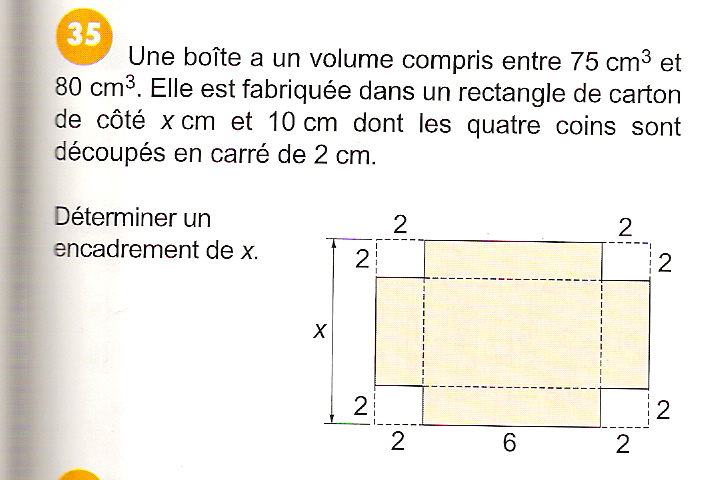
\includegraphics[width=8cm]{images/ex35.jpg}
\end{center}
	  \textit{Remarque:} On peut fabriquer le patron pour comprendre le calcul
	  du volume.

\bigskip
\textbf{Exercice 3:}
\begin{center}
	  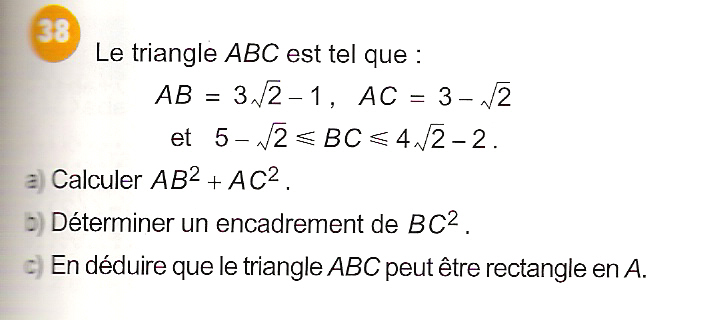
\includegraphics[width=8cm]{images/ex38.jpg}
\end{center}


\bigskip
\textbf{Exercice 4:} Soit $x$ un r�el strictement sup�rieur � $3$. L'aire du
rectangle de c�t�s $x+1$ et $x-3$ est  strictement inf�rieure � l'aire du carr�
de c�t� $x-2$. D�terminer les valeurs possibles de $x$. Donner l'ensemble
solution sous forme d'intervalles.

\bigskip
\textbf{Exercice 5:} (facultatif) Pour $2$ points de plus \ldots\\
$x$ et $y$ sont des entiers strictement positifs tel que $x<y$. Comparer les
nombres $\dfrac{x-1}{x}$ et $\dfrac{y-1}{y}$.

\newpage

\textbf{NOM Pr�nom:} \ldots \ldots \ldots \ldots \ldots \ldots
\bigskip
\bigskip


\begin{tabular}{|m{35mm}|c|m{35mm}|m{35mm}|m{35mm}|}
\hline
Texte & Intervalles & Repr�sentation sur une droite gradu�e & Ensemble
des r�els $x$ v�rifiant: & L'ensemble est-il born�? (oui ou non)\\
\hline
& & 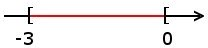
\includegraphics[width=3cm]{images/ex11.jpg} & & \\[7mm]
\hline
& & & $\dfrac{-5}{3}\leqslant x \leqslant \dfrac{-10}{7}$ & \\[7mm]
\hline
& & 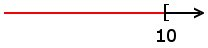
\includegraphics[width=3cm]{images/ex12.jpg} & & \\[7mm]
\hline
l'ensemble des r�els positifs ou nuls & & & & \\[7mm]
\hline
& $]-\infty;7]$ & & & \\[7mm]
\hline
l'ensemble des r�els compris strictement entre $-10$ et $-2$ & & & & \\[7mm]
\hline
& & & $x<0$ & \\[7mm]
\hline
l'ensemble des r�els sup�rieurs ou �gaux � -4 & & & & \\[7mm]
\hline
& $]7;-\infty[$ & & & \\[6mm]
\hline
\end{tabular}

\end{document}
